\subsection{Diffuse lighting}
When calculating the diffuse lighting in a single point in the phong shading
process, we estimate that the intensity of the light that is reflected does not
vary depending on the position from which the point is viewed. This is also
referred to as a lambertian reflectance. As our light source is of the type
'point' we use the following formula to calculate the reflection of light in a
single point on the surface:

$$I_{diffuse}(x) = Li(x) Kd(x) max(n(x) · l(x), 0)$$ $Li$ is the intensity of
the light source. The light intensity decreases as we move farther away from
the source. This is calculated through $$Idiffuse(x) = Il(x) kd(x) max(n(x) ·
l(x), 0)$$
 In our model we assume that the light intensity does not decrease.
$Kd$ is the properties of the Lambertian surface. As some surfaces reflects
light more than others (ranging from perfect mirrors to total absorption of the
light), this property dictates how much of the light is reflected.

The $max(n(x) · l(x), 0)$ part finds the dot product between the light vector
and the normal in the point. If this value is less than zero, the angle between
the two is large enough for the light source to be behind the surface. As a
result the lighting value is set to zero (as all previous values are multiplied
by this factor). This makes sense, as as surface lit from behind would not
receive any direct illumination. The technique used is similar to the one used
in back face culling, where we also measure the normal. The difference between
the two being that in culling we used the vector from the camera to the
surface, and here we use the vector from the light source to the surface-point. 

\begin{figure}[H]
    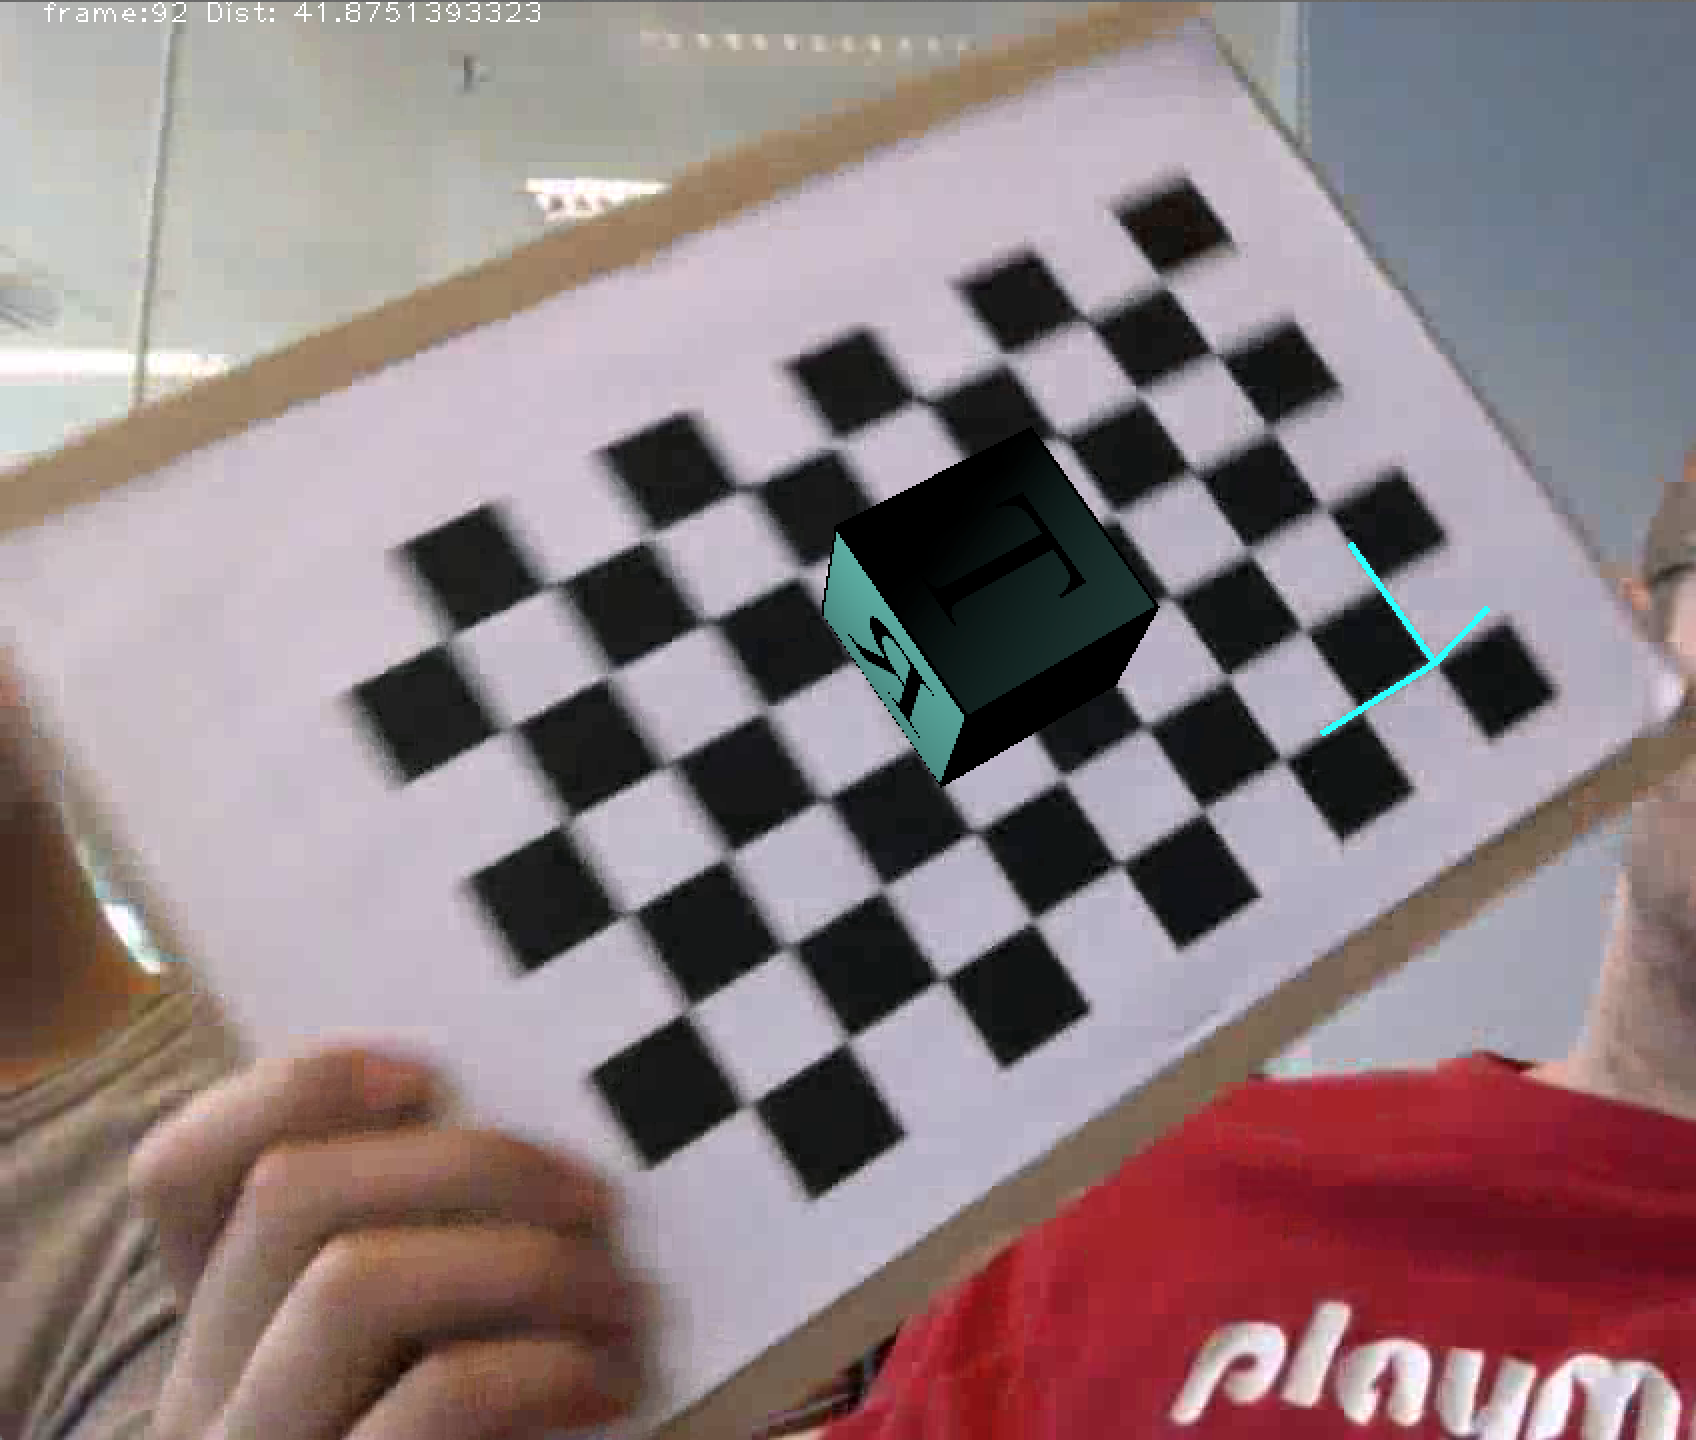
\includegraphics{pics/phongDiffuseOnly.png}
    \label{fig:EphongDiffuseOnly}
    \caption{\textbf{Example of lambertian surfaces with diffuse lighting.} 
    the diffuse light makes a huge difference in conveying the illusion of depth. Although for realistic looking lights we also need the ambient and specular light. }
\end{figure}